\documentclass[12pt, letterpaper, titlepage]{article}

\usepackage{amsmath}
\usepackage{booktabs}
\usepackage{amsthm}
\usepackage{graphicx}
\usepackage[margin=1in]{geometry}
\usepackage{hyperref}
\hypersetup{colorlinks = true, linkcolor = blue, citecolor=blue, urlcolor = blue}
\usepackage{natbib}
\usepackage{enumitem}
\usepackage{setspace}

\usepackage[pagewise]{lineno}
\linenumbers*[1]
% %% patches to make lineno work better with amsmath
\newcommand*\patchAmsMathEnvironmentForLineno[1]{%
 \expandafter\let\csname old#1\expandafter\endcsname\csname #1\endcsname
 \expandafter\let\csname oldend#1\expandafter\endcsname\csname end#1\endcsname
 \renewenvironment{#1}%
 {\linenomath\csname old#1\endcsname}%
 {\csname oldend#1\endcsname\endlinenomath}}%
\newcommand*\patchBothAmsMathEnvironmentsForLineno[1]{%
 \patchAmsMathEnvironmentForLineno{#1}%
 \patchAmsMathEnvironmentForLineno{#1*}}%

\AtBeginDocument{%
 \patchBothAmsMathEnvironmentsForLineno{equation}%
 \patchBothAmsMathEnvironmentsForLineno{align}%
 \patchBothAmsMathEnvironmentsForLineno{flalign}%
 \patchBothAmsMathEnvironmentsForLineno{alignat}%
 \patchBothAmsMathEnvironmentsForLineno{gather}%
 \patchBothAmsMathEnvironmentsForLineno{multline}%
}

\newcommand{\jy}[1]{\textcolor{blue}{JY: #1}}

\title{On Misuses of the Kolmogorov–-Smirnov Test for One Sample Goodness-of-Fit}

\author{Anthony Zeimbekakis and Jun Yan\\
\href{mailto:anthony.zeimbekakis@uconn.edu}{\nolinkurl{anthony.zeimbekakis@uconn.edu}}\\
Department of Statistics, University of Connecticut}
\date{April 21, 2022}

\begin{document}
\maketitle

\doublespace

\begin{abstract}
The Kolmogorov--Smirnov (KS) test is one the most popular goodness-of-fit tests for 
comparing a sample with a hypothesized parametric distribution. Nevertheless, it has 
often been misused. The standard one-sample KS test applies to independent, continuous 
data with a hypothesized distribution that is completely specified. It is not uncommon, 
however, to see in the literature that it was applied to dependent, discrete, or 
rounded data, with hypothesized distributions containing estimated parameters. 
For example, it has been ``discovered'' multiple times that the test is too conservative 
when the parameters are estimated. We demonstrate
misuses of the one-sample KS test in three scenarios through simulation studies:
1) the hypothesized distribution has unspecified parameters;
2) the data are serially dependent; and
3) a combination of the first two scenarios.
For each scenario, we provide remedies for practical applications.
\end{abstract}

\jy{keep line width under 80 characters in tex source}

\section{Introduction}\label{sec:intro}

The Kolmogorov-Smirnov (KS) statistic is one of the most popular goodness-of-fit 
tests for comparing a sample with a hypothesized parametric distribution.
Let $X_1, ..., X_n$ be a random sample from some continuous
distribution. The null hypothesis $H_0$ is that the population distribution is $F$.
Let $F_n(\cdot)$ be the empirical cumulative distribution. The KS statistic is
\[
  D = \sup_x {\lvert F_{n}(x) - F(x) \rvert}.
\]
\jy{use upper case for random variables}
The distribution of $D$ under $H_0$ turned out to be independent of the
distribution $F$ and  table of critical values for $D$ has been constructed
\citet{Massey} for various sample sizes $n$ and significance 
levels $\alpha$. If the value of $d$ exceeds the test's corresponding critical value, 
the null hypothesis is rejected. The KS test is available in popular statistical
software packages, such as function \texttt{ks.test} in R \citep{R}.
\jy{cite R and also some of the references on the help page of the function}


The standard one-sample KS test applies to independent data with a continuous
hypothesized distribution that is completely specified.
\jy{this paragraph needs some reorganization.
  Flow: not applicable to discrete or rounded data (give references; which is
  not the focus of this paper);
  not applicable to fitted distributions;
  not applicable to serially dependent data}
\jy{break the big paragraph into smaller ones}
Often in literature, it has been "discovered" that the test loses its power when 
applied to dependent or discrete data with hypothesized distributions containing 
estimated parameters. In the case of estimated parameters, \citet{Steinskog} 
demonstrates the change in power when using estimated parameters and stress caution in 
using the KS test in such ways. \citet{Lilliefors} shows 
that using the standard table when values of the mean and standard deviation are 
estimated obtains extremely conservative results. This is supported by \citet{Capasso}, which 
concludes that failing to re-estimate the parameters may lead to wrong, overly-conservative 
approximations to the distributions of goodness-of-fit test statistics based on the empirical 
distribution function. \citet{Capasso} also notes that the impact of this possible mistake 
may turn out to be dramatic and does not vanish as the sample size increases. Remedies are provided 
by \citet{Genest} and \citet{Babu} in the form of bootstrap. \citet{Genest} provides validity 
for using parametric bootstrap with various goodness-of-fit tests. \citet{Babu} details 
the bootstrap procedure for goodness-of-fit tests and notes that both parametric and 
non-parametric procedures lead to correct asymptotic levels, however there is a correction 
required for the non-parametric case. In the case of dependent data, \citet{Durilleul} demonstrates
that the KS statistic is too liberal for medium-to-high positive autocorrelation values. 
\citet{Durilleul} also shows that for negative autocorrelation values, the behavior is 
asymmetrical with respect to positive values. For remedies, \citet{Weiss} provides a 
procedure that is applicable specifically for data modeled by the second-order auto-regressive (AR) 
process where the parameters are known. \citet{Lanzante} tests various strategies for dealing with 
temporal dependence and concludes that a test based on Monte-Carlo simulations performed the best.
We propose a bootstrap procedure involving copulas to account for dependence.


The contribution of this paper is a demonstration of misuses of the one-sample
KS test in three scenarios and their remedies in practice. In order to set 
up the demonstrations, simulated data is used throughout. Unless otherwise specified, 
the random data is generated from a standard normal distribution with sample size $n = 100$. 
Therefore the cumulative distribution $F(x)$ of the KS test for much of this paper is standard normal.
\jy{Let's not restrict to normal distributions.}

The rest of the paper is organized as follows. Section~\ref{sec:fitted}
investigates the scenario where the hypothesized distribution has an unspecified
parameters. Both parametric and nonparametric bootstrap are available to fix the
issue. Section~\ref{sec:dependence} ... ... \jy{fill this}
Section~\ref{sec:conclusion} concludes with a discussion.

\section{Fitted Parameters}\label{sec:fitted}

The null distribution of the KS statistic changes when the hypothesized
distribution contains fitted parameters. In this scenario, the null hypothesis
is $H_0$: the random sample $X_1, \ldots, X_n$ come from a continuous
distribution $F_{\theta}$ with unspecified parameter $\theta$.
Let $\hat\theta_n$ be an estimator of $\theta$, which could be, for example,
maximum likelihood estimator of moment estimator. The test statistic is
\[
  D = \sup_x | F_n(x) - F_{\hat\theta_n}(x) |.
\]
Because $F_{\hat\theta_n}$ is not the same as the true data generating
$F_\theta$, the null distribution of $D$ obtained in existing implementations in
software packages which assumes completely known $F_\theta$ no long applies.
\jy{cite the paper that ``rediscovered'' the fact}


For illustration, \jy{give the details of the setting}
However, the procedure is sometimes performed where the population cumulative 
distribution $F(x)$ has parameters $\mu=\bar X$, the sample mean, and $\sigma^2=s^2$, 
the sample variance \citep{Lilliefors}. This case is demonstrated in Figure~\ref{fig:hist_fitted} 
under the Naive plot. The naive KS test was performed by estimating the parameters 
of $F(x)$ using the fitted distribution of the sample data. Since the data is generated 
from a standard normal distribution with seemingly all assumptions met, a uniform 
distribution of $U(0,1)$ is expected for the p-values. However this is under the 
assumption that the KS test holds its power, which it no longer does due to using 
fitted parameters. Therefore, there is notable deviation from the uniform distribution. 


To fix the problem, parametric bootstrap can be used to approximate the null
distribution of the testing statistic. 
\begin{enumerate}
  \item 
    Draw a random sample $X_1^*,...,X_n^*$ from the fitted distribution $F_{\hat\theta_n}$
  \item 
    Fit $F_\theta$ to the sample and obtain estimated $\hat\theta_n^*$
  \item
    Obtain the empirical distribution function of the random sample $F_n^*$
  \item 
    Calculate bootstrap KS statistic
    \[
      D^* = \sup_x \lvert F_n^* (x)- F_{\hat\theta_n}^*(x) \rvert.
    \]
  \item
    Repeat the previous steps a large number $B$ times and use the empirical
    distribution of the $B$ test statistics as an approximate distribution of
    the null distribution of the observed statistic.      
\end{enumerate}


% In parametric bootstrap, the resampling is done where $\hat{F}_n = F(.;\hat{\theta}_n)$. 
% Bootstrap samples are drawn from ${F}(.,\hat{\theta}_n)$ where the assumed distribution 
% $F$ is normal and $\hat{\theta}_n = (\bar X, s)$, the sample mean and sample standard 
% deviation. For each bootstrap sample, a KS test statistic is found using those 
% fitted parameters.

\jy{for clarity, give the steps of the nonparametric bootstrap procedure and
  make clear the bias correction step.}

In non-parametric bootstrap, the resampling is done where $\hat{F}_n = F_n$. The non-parametric
case requires a correction for bias detailed by \citet{Babu}. There is a known bias
term $B_{n}(x) = \sqrt{n}(F_{n}(x) - F(x;\hat{\theta}_n)$. Including this term in the
calculation of the KS statistic corrects the bias \citet{Babu}:
$d = \max\lvert F_{n}(x) - F(x) - B_{n}(x) \rvert$.


\begin{figure}[tbp]
  \centering
  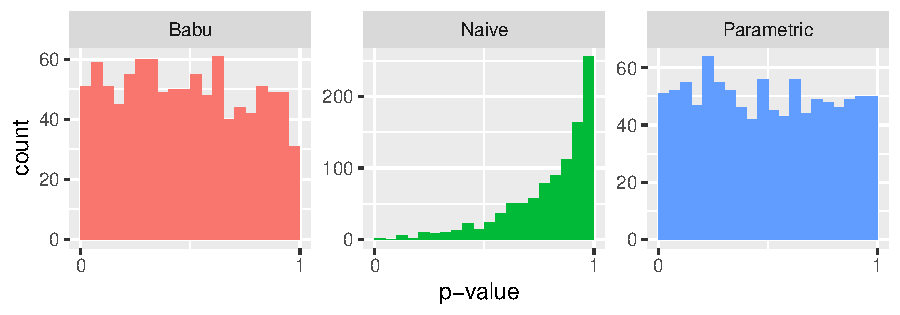
\includegraphics[width=\textwidth]{hist_fitted}
  \caption{Histograms demonstrating fitted parameters. \jy{make the caption self-contained.}}
  \label{fig:hist_fitted}
\end{figure}

Figure~\ref{fig:hist_fitted} displays the results of from our simulations. The procedure 
is replicated $1000$ times using the standard normal distribution with sample size $n=100$. 
In each replicate test, $1000$ bootstrap samples are obtained. The p-value can be calculated
by counting the number of bootstrap KS statistics greater than or equal to the observed KS statistic, 
and then dividing by the number of bootstrap samples. It is clear from the figure that both
bootstrap processes correct for the problem of fitted parameters. The plots appear to be
$U(0,1)$, which is expected of a full power test.

\section{Serially Dependent Data}\label{sec:dependence}

The KS test also displays issues in the case of dependence. As mentioned, an assumption of the 
test is that the data is independent. Unfortunately, real data is often temporally
or spatially dependent and the results of a goodness-of-fit test would be valuable. 
When the KS test is performed on dependent data it performs poorly. This is demonstrated
with a simulation in Figure~\ref{fig:hist_correlation}. Data is generated from a
\jy{give more details about the simulation setting: what ar1 coefficients were
  considered? What was the null hypothesis? How was the test statistic calculated?}
first-order autoregressive model (AR(1)) with a standard normal distribution. The simulation
is done with the levels of $\psi$ varying from $(-3,3)$. The results echo those of \citet{Durilleul}
that the KS statistic is too liberal for positive autocorrelation values, and 
that the behavior is asymmetrical for negative values.

\begin{figure}[tbp]
  \centering
  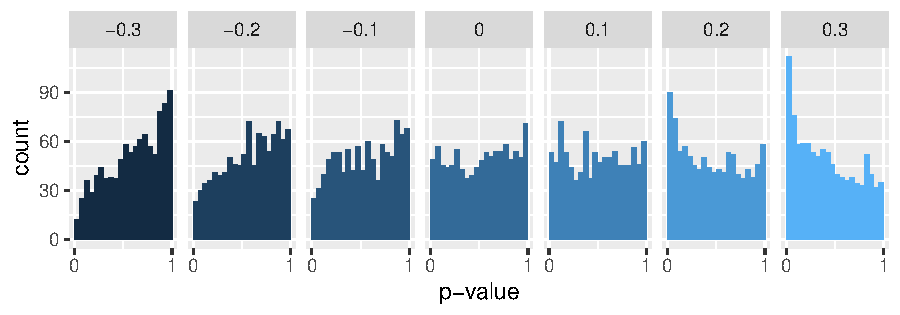
\includegraphics{hist_correlation}
  \caption{Histograms of P-values with correlated data.}
  \label{fig:hist_correlation}
\end{figure}

In order to correct this, we can employ a parametric bootstrap procedure which
assumes a working serial dependence structure through copulas. A copula is a
multivariate distribution with standard uniform marginal distributions, which
completely characterizes the dependence structure of a multivariate
distribution \cite{copula, book}. For simplicity, we assume a normal copula with
an AR-1 structure to characterize the serial dependence of the observations. The
AR-1 parameter of the normal copula is set to match the be the sample serial
Spearman's rho of the observed sample. The procedure is as follows.


\begin{enumerate}
  \item Calculate the observed KS statistic \jy{the observed statistic is
      calculated the same way still, so it is not needed in the algorithm here}
  \item Get the lag-1 sample auto-spearman rho
  \item Perform parametric bootstrap to get an empirical distribution of the KS
    statistic
    \jy{need to spell out the details; how to generate $X_t$ given $X_{t-1}$?}
\end{enumerate}


\jy{add a discussion about the method. The method is exact if the true
  dependence is indeed a normal copula with an ar1 structure. When it is not, it
  may still give a reasonable approximation that can be useful for practical purpose}

\begin{figure}[tbp]
  \centering
  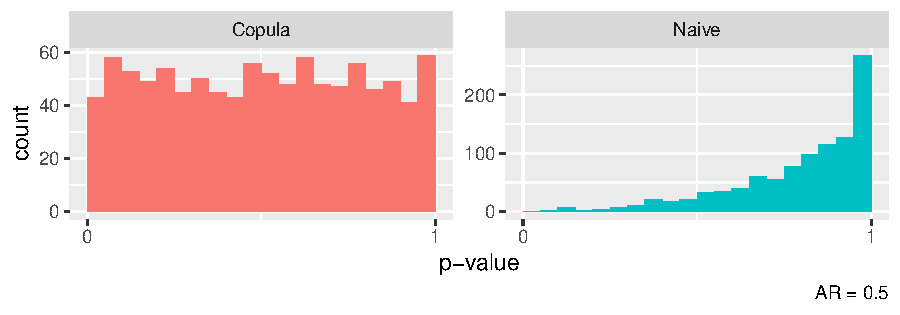
\includegraphics{hist_copula_only}
  \caption{Histograms demonstrating copula use to correct dependence.}
  \label{fig:hist_copula_only}
\end{figure}

Figure~\ref{fig:hist_copula_only} displays the results of the copula remedy for dependent data.
The data is generated from an AR(1) model with $\psi = .5$. The copula used is to model
dependence is the normal copula. $1000$ replicate tests were performed with
$1000$ bootstrap samples per test.
\jy{present other scenarios too}
The naive test is performed by simply using the KS test without correcting for any 
potential dependence.


\section{Fitted Parameters and Serially Dependent Data}\label{sec:fittedwithdependence}

\jy{give a stronger motivation; last section is not practical at all because we
  often don't know the parameters; this section combines the last two}
The remedy using copulas is effective in the case where both assumptions are violated.
This is shown in Figure~\ref{fig:hist_copula}. The ``super naive" method is the resulting 
p-values when you naively use fitted parameters while ignoring dependence in the data.
The ``naive parametric" plot is the result of applying parametric bootstrap to correct
for fitted parameters while ignoring potential dependence. Of course, the "copula" 
plot applies the fix for both assumptions. The results show that copula remedy generates 
uniform p-values and restores the power of the KS test.

\begin{figure}[tbp]
  \centering
  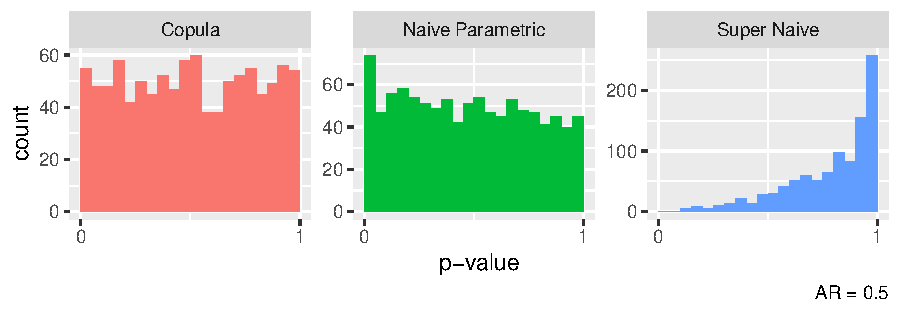
\includegraphics{hist_copula}
  \caption{Histograms demonstrating copula use to correct fitted parameters and dependence.}
  \label{fig:hist_copula}
\end{figure}

The copula fix is not a complete solution, because regardless of the true dependence in the data
we assume an AR(1) model by taking the lag-1 sample auto-spearman rho. However, we can 
show that as long as the AR(1) assumption is a close approximation, the correction still restores power to the test.
Figure~\ref{fig:hist_copula_ma1} is the procedure performed on data generated from 
an MA(1) model with $\theta = 0.5$. Figure~\ref{fig:hist_copula_arma} displays results with 
data generated from an ARMA(1,1) model with $\psi = 0.5$ and $\theta = 0.3$. 

\begin{figure}[tbp]
  \centering
  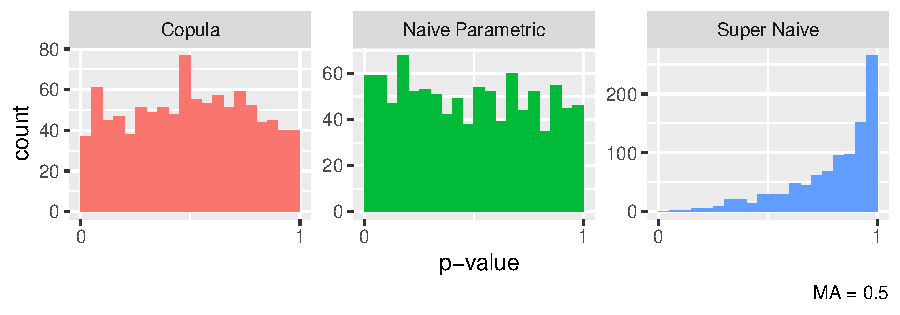
\includegraphics{hist_copula_ma1}
  \caption{Histograms demonstrating remedy use with MA(1) model.}
  \label{fig:hist_copula_ma1}
\end{figure}

\begin{figure}[tbp]
  \centering
  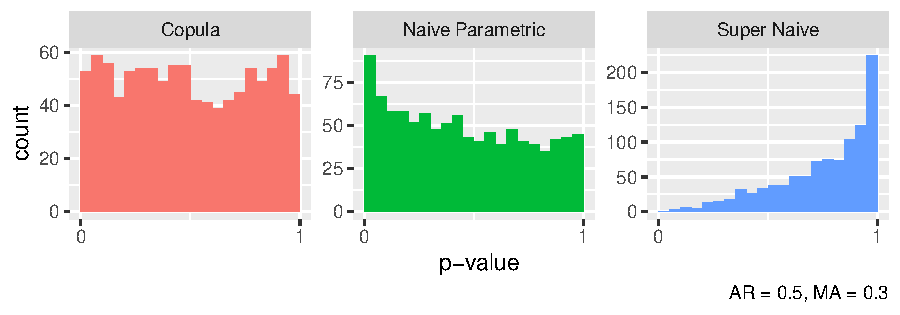
\includegraphics{hist_copula_arma}
  \caption{Histograms demonstrating remedy use with ARMA(1,1) model.}
  \label{fig:hist_copula_arma}
\end{figure}

It is also possible to apply our procedure to other distributions. All of the simulations
to this point have been done with standard normal data. The data in Figure~\ref{fig:hist_copula_gamma} 
is generated from $Gamma ~ (3,1)$ with a correlation coefficient of $\rho = 0.5$. Figure~\ref{fig:hist_copula_gev}
shows the procedure applied to data from $GEV ~ (0, 0.2, 1)$ with a correlation coefficient of $\rho = 0.5$. 

\begin{figure}[tbp]
  \centering
  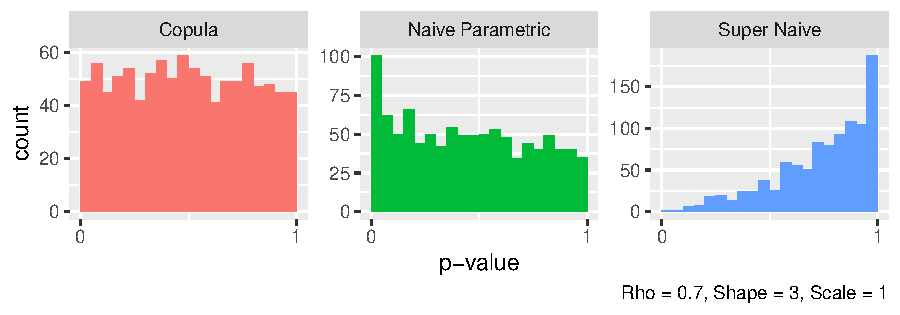
\includegraphics{hist_copula_gamma}
  \caption{Histograms demonstrating remedy with Gamma(3,1).}
  \label{fig:hist_copula_gamma}
\end{figure}

\begin{figure}[tbp]
  \centering
  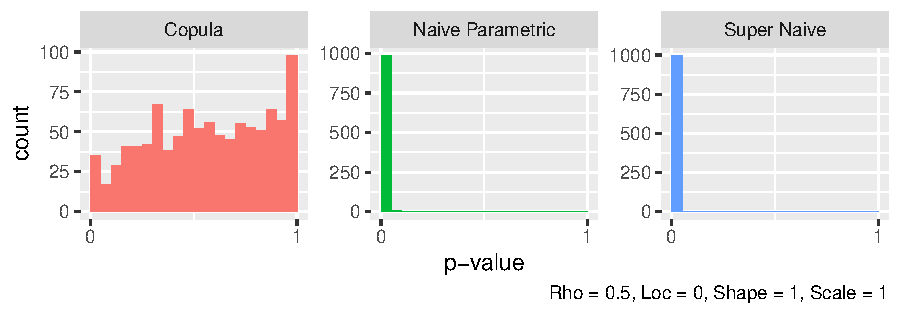
\includegraphics{hist_copula_gev}
  \caption{Histograms demonstrating copula use to correct dependence.}
  \label{fig:hist_copula_gev}
\end{figure}

Where this remedy falls short is when the approximation of an AR(1) model is too inaccurate.
An AR(2) model can be used to demonstrate this. For an AR(2) model with $\phi = (0.5, 0.3)$,
Figure~\ref{fig:hist_copula_ar2} displays the results of applying the various remedies. 
While the remedies improve the plot of the p-values in comparison to the naive case,
because the approximation is not close enough the correction does not work completely.

\begin{figure}[tbp]
  \centering
  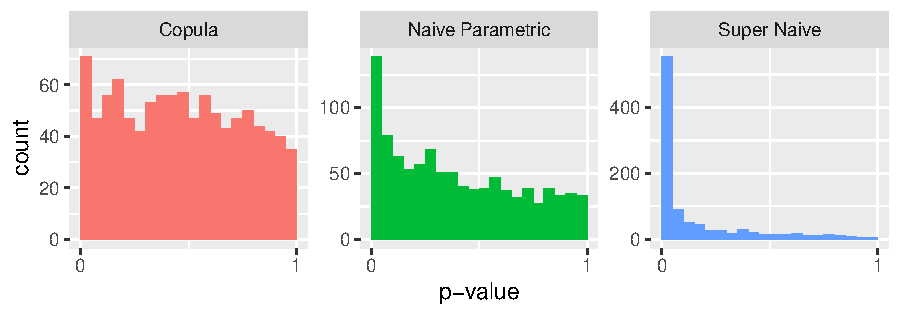
\includegraphics{hist_copula_ar2}
  \caption{Histograms demonstrating copula use to correct dependence.}
  \label{fig:hist_copula_ar2}
\end{figure}


\section{Conclusion}\label{sec:conclusion}

The KS test has base assumptions that the hypothesized distribution is completely specified
and the data is independent. When these assumptions are violated, the test is no
longer accurate and remedies must be performed. In the case of fitted parameters, 
parametric and non-parametric bootstrap can restore the power of the test. A bias 
correction is required if the non-parametric form is used \citep{Babu}. In the case of dependent
data, a procedure using bootstrap with copulas to model dependency shows positive results.
When both assumptions are violated, that is the case where the data has dependence and 
parameters must be fitted, the copula remedy also shows positive results. The tests were 
performed on simulated data from a standard normal distribution, though also appear effective
against other distributions such as gamma and gev. The copula remedy
is not a complete solution. Regardless of the true dependence, we use an AR(1) model.
Therefore, if the AR(1) model is a close approximation of the truth, the fix can work.
However, in cases such as AR(2), the approximation is incorrect and the fix does not 
completely restore power.


\bibliographystyle{chicago}
\bibliography{citations.bib}


\end{document}
